\begin{frame}{$K^0$ previous result}
  \begin{tabular}{cc}
    \begin{minipage}{0.4\hsize}
      \begin{figure}
        \scriptsize
        Acceptance\\
        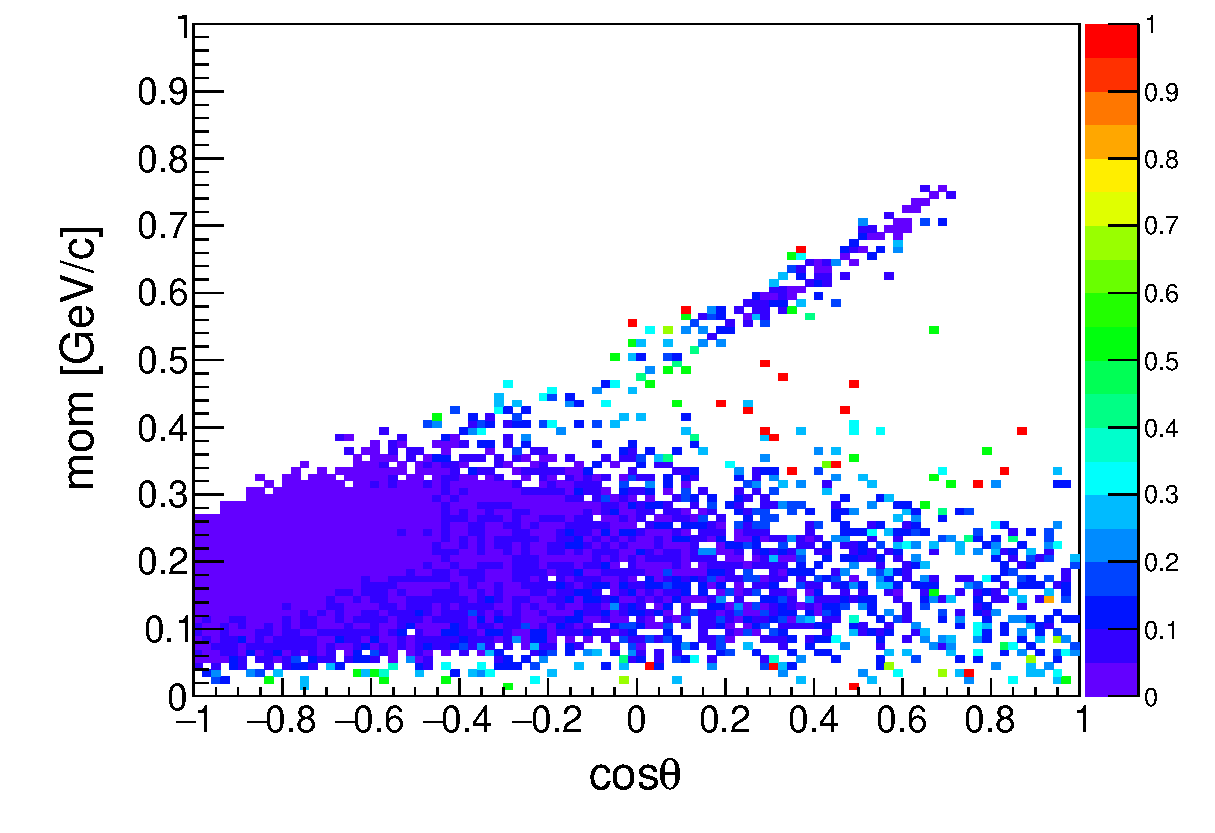
\includegraphics[width=2.5cm]{../pic/Run78/QE/K0_cos_mom_acc.eps}
      \end{figure}
      \begin{tabular}{cc}
        \begin{minipage}{0.5\hsize}
          \begin{figure}
            \scriptsize
            Before correction
            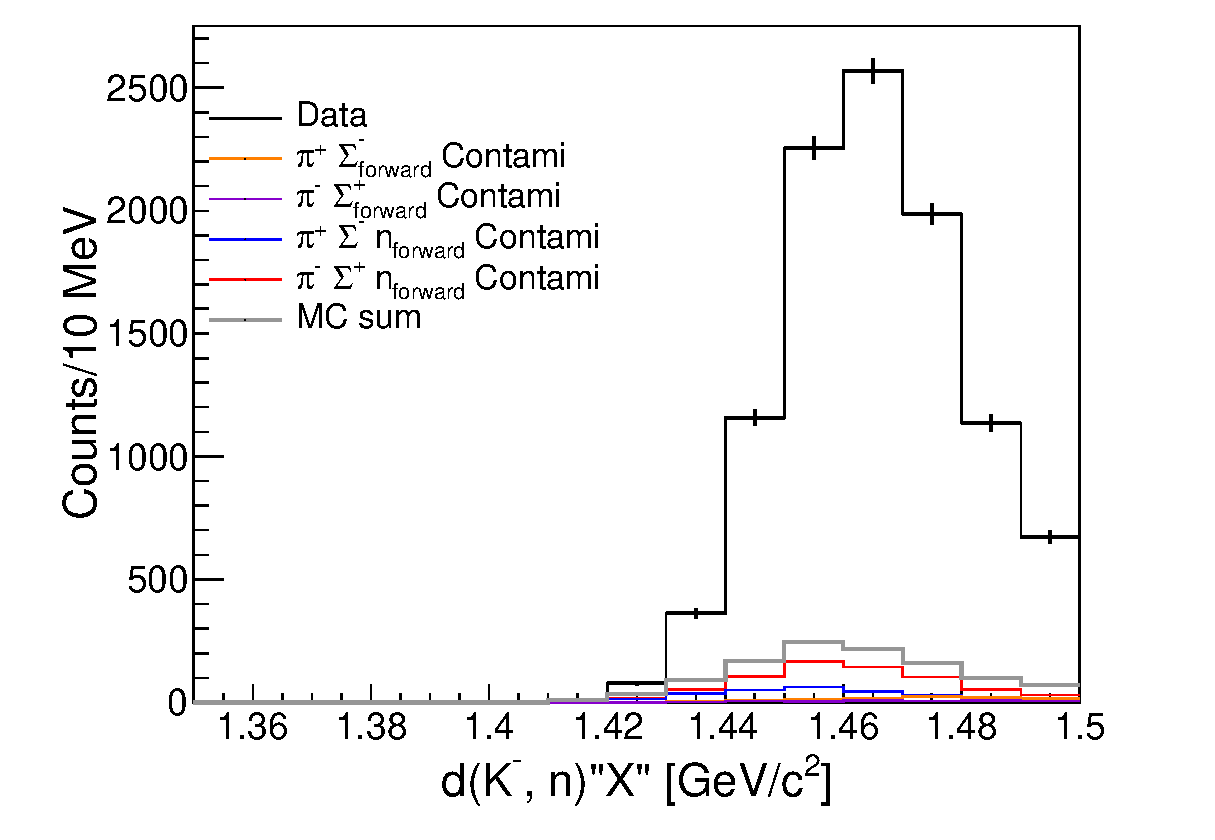
\includegraphics[width=2.5cm]{../pic/Run78/QE/KN_MM_wK0_tag.eps}
          \end{figure}
        \end{minipage}

        \begin{minipage}{0.5\hsize}
          \begin{figure}
            \scriptsize
            After correction
            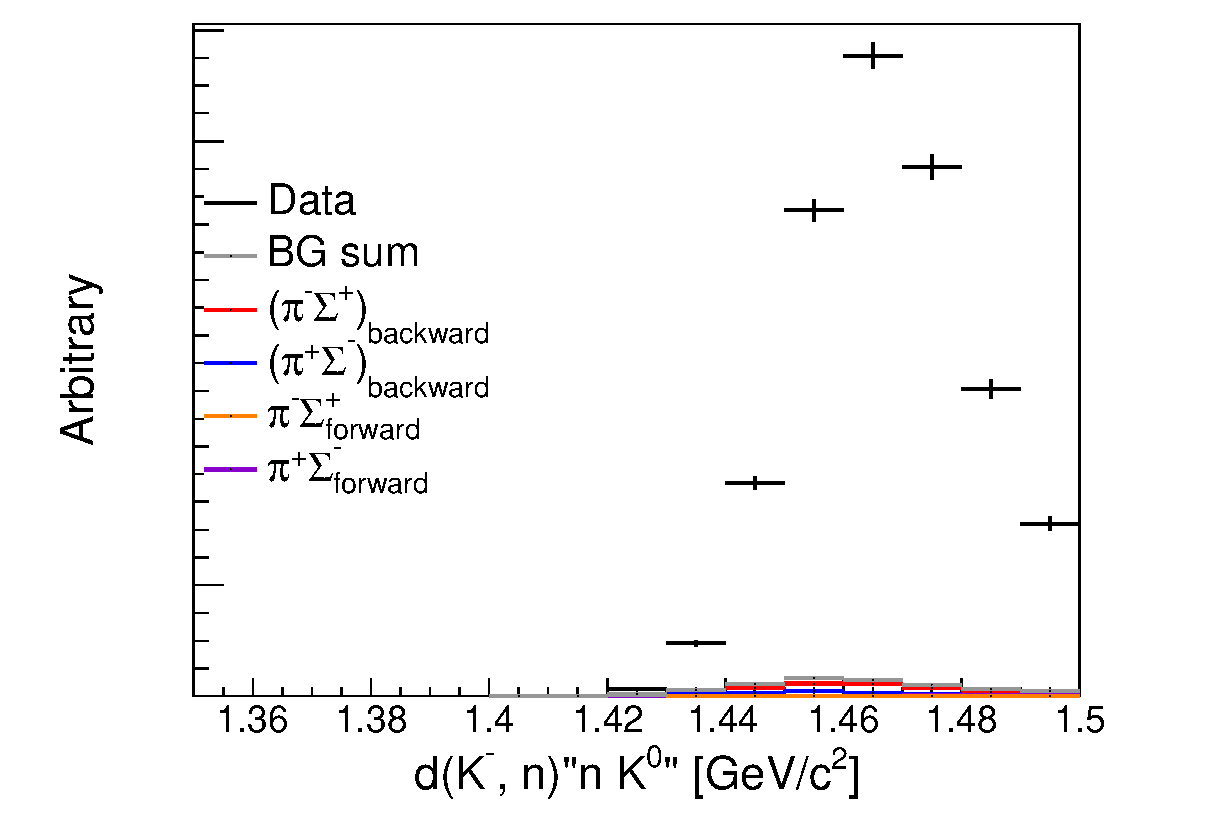
\includegraphics[width=2.5cm]{../pic/Run78/QE/K0_spec_wBG.eps}
          \end{figure}
        \end{minipage}
      \end{tabular}
    \end{minipage}

    \begin{minipage}{0.6\hsize}
      \begin{figure}
        $K^0$ Cross Section\\
        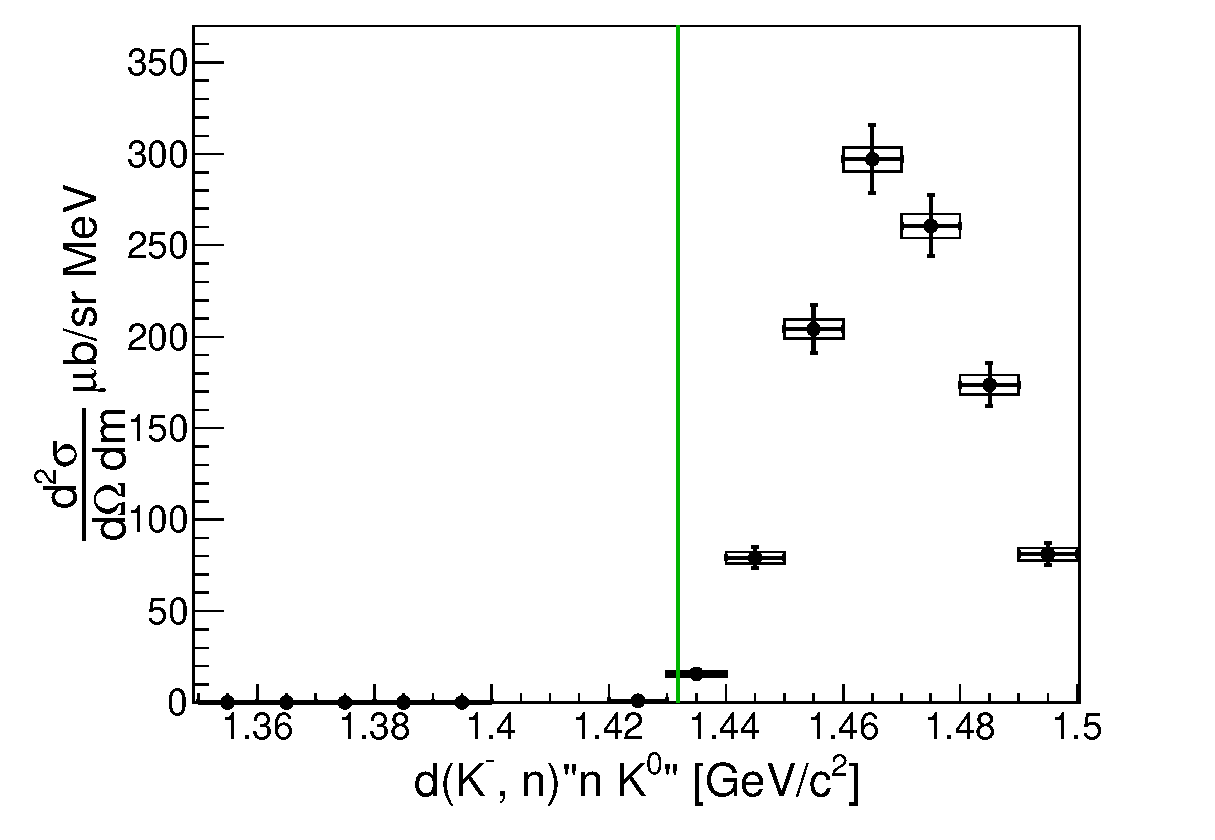
\includegraphics[width=6cm]{../pic/Run78/QE/K0_CS.eps}
      \end{figure}
      \vspace{-5mm}
      \centering
      \scriptsize
      Background processes were subtracted.\\
      Boxes indicate statisical errors.\\
      Error bars include scaling factor.
    \end{minipage}
  \end{tabular}
  \centering
  \footnotesize
  \vspace{3mm}\\
  $d(K^-, n)"n K^0"$ spectrum looks like quasi-elastic (1-step).\\
  Cross Section was converted by acceptance of $\cos\theta$ and mom of $K^0$.
  \begin{equation*}
    \frac{d^2\sigma}{d\Omega dM_{d(K^-, n)}}=F\times \sum M(\cos\theta, p)\times\frac{1}{A(\cos\theta, p)}
  \end{equation*}

\end{frame}
